% !TEX TS-program = xelatex
% !BIB program = bibtex
% !TeX spellcheck = ru_RU

% About magic macroses see also
% https://tex.stackexchange.com/questions/78101/

% По умолчанию используется шрифт 14 размера. Если нужен 12-й шрифт, уберите опцию [14pt]
\documentclass[14pt, russian]{matmex-diploma-custom}

% !TeX spellcheck = ru_RU
% !TEX root = vkr.tex
% Опциональные добавления используемых пакетов. Вполне может быть, что они вам не понадобятся, но в шаблоне приведены примеры их использования.
\usepackage{tikz} % Мощный пакет для создание рисунков, однако может очень сильно замедлять компиляцию
\usetikzlibrary{decorations.pathreplacing,calc,shapes,positioning,tikzmark}

% Библиотека для TikZ, которая генерирует отдельные файлы для каждого рисунка
% Позволяет ускорить компиляцию, однако имеет свои ограничения
% Например, ломает пример выделения кода в листинге из шаблона
% \usetikzlibrary{external}
% \tikzexternalize[prefix=figures/]

\newcounter{tmkcount}

\tikzset{
  use tikzmark/.style={
    remember picture,
    overlay,
    execute at end picture={
      \stepcounter{tmkcount}
    },
  },
  tikzmark suffix={-\thetmkcount}
}

\usepackage{booktabs} % Пакет для верстки "более книжных" таблиц, вполне годится для оформления результатов
% В шаблоне есть команда \multirowcell, которой нужен этот пакет.
\usepackage{multirow}
\usepackage{siunitx} % для таблиц с единицами измерений

\newcommand{\cd}[1]{\texttt{#1}}
\newcommand{\inbr}[1]{\left<#1\right>}

% Для названий стоит использовать \textsc{}
\newcommand{\OCaml}{\textsc{OCaml}}
\newcommand{\miniKanren}{\textsc{miniKanren}}
\newcommand{\BibTeX}{\textsc{BibTeX}}
\newcommand{\vsharp}{\textsc{V$\sharp$}}
\newcommand{\fsharp}{\textsc{F$\sharp$}}
\newcommand{\csharp}{\textsc{C$\sharp$}}
\newcommand{\GitHub}{\textsc{GitHub}}
\newcommand{\SMT}{\textsc{SMT}}

\newcolumntype{L}[1]{>{\raggedright\let\newline\\\arraybackslash\hspace{0pt}}m{#1}}
%\newcolumntype{C}[1]{>{\centering\let\newline\\\arraybackslash\hspace{0pt}}m{#1}}
\newcolumntype{R}[1]{>{\raggedleft\let\newline\\\arraybackslash\hspace{0pt}}m{#1}}

\usepackage{xcolor}

%  Команды и пакеты, не используемые в шаблоне, которые тем не менее могут быть полезными.

% \newcolumntype{Y}{>{\centering\arraybackslash}X}

% \usepackage{mathrsfs}

\lstdefinestyle{fsharp}{
  basicstyle=\small\ttfamily,
  keywordstyle=\color{blue},
  commentstyle=\color{lightblue},
  stringstyle=\color{red},
  numbers=left,
  numberstyle=\tiny\color{gray},
  stepnumber=1,
  numbersep=10pt,
  backgroundcolor=\color{white},
  showspaces=false,
  showstringspaces=false,
  showtabs=false,
  tabsize=2,
  breaklines=true,
  breakatwhitespace=false,
  morekeywords={async, let, rec, if, then, else, do, yield, return, use, match, with, function}
  literate={->}{{$\to$}}3 {==}{{$\equiv$}}1 {=/=}{{$\not\equiv$}}1 {|>}{{$\triangleright$}}3 {\\/}{{$\vee$}}2 {/\\}{{$\wedge$}}2 {>=}{{$\ge$}}1 {<=}{{$\le$}}
}


\usepackage{totcount}

\begin{document}
% TODO: Formatting
% !TeX spellcheck = ru_RU
% !TEX root = vkr.tex

%% Если что-то забыли, при компиляции будут ошибки Undefined control sequence \my@title@<что забыли>@ru
%% Если англоязычная титульная страница не нужна, то ее можно просто удалить.
\filltitle{ru}{
    %% Актуально только для курсовых/практик. ВКР защищаются не на кафедре а в ГЭК по направлению,
    %%   и к моменту защиты вы будете уже не в группе.
    chair              = {Кафедра системного программирования},
    group              = {22.Б07-мм},
    %
    %% Макрос filltitle ненавидит пустые строки, поэтому обязателен хотя бы символ комментария на строке
    %% Актуально всем.
    title              = {Реализация процедурной генерации интерьера комнат в 3D-игре на Unity},
    %
    %% Здесь указывается тип работы. Возможные значения:
    %%   production - производственная практика;
    %%   coursework - отчёт по курсовой работе;
    %%   practice - отчёт по учебной практике;
    %%   prediploma - отчёт по преддипломной практике;
    %%   master - ВКР магистра;
    %%   bachelor - ВКР бакалавра.
    type               = {practice},
    %
    %% Здесь указывается вид работы. От вида работы зависят критерии оценивания.
    %%   solution - <<Решение>>. Обучающемуся поручили найти способ решения проблемы в области разработки программного обеспечения или теоретической информатики с учётом набора ограничений.
    %%   experiment - <<Эксперимент>>. Обучающемуся поручили изучить возможности, достоинства и недостатки новой технологии, платформы, языка и т. д. на примере какой-то задачи.
    %%   production - <<Производственное задание>>. Автору поручили реализовать потенциально полезное программное обеспечение.
    %%   comparison - <<Сравнение>>. Обучающемуся поручили сравнить несколько существующих продуктов и/или подходов.
    %%   theoretical - <<Теоретическое исследование>>. Автору поручили доказать какое-то утверждение, исследовать свойства алгоритма и т.п., при этом не требуя написания кода.
    kind               = {production},
    %
    author             = {САВЕЛЬЕВА Полина Андреевна},
    %
    %% Актуально только для ВКР. Указывается код и название направления подготовки. Типичные примеры:
    %%   02.03.03 <<Математическое обеспечение и администрирование информационных систем>>
    %%   02.04.03 <<Математическое обеспечение и администрирование информационных систем>>
    %%   09.03.04 <<Программная инженерия>>
    %%   09.04.04 <<Программная инженерия>>
    %% Те, что с 03 в середине --- бакалавриат, с 04 --- магистратура.
    specialty          = {02.03.03 <<Математическое обеспечение и администрирование информационных систем>>},
    %
    %% Актуально только для ВКР. Указывается шифр и название образовательной программы. Типичные примеры:
    %%   СВ.5006.2017 <<Математическое обеспечение и администрирование информационных систем>>
    %%   СВ.5162.2020 <<Технологии программирования>>
    %%   СВ.5080.2017 <<Программная инженерия>>
    %%   ВМ.5665.2019 <<Математическое обеспечение и администрирование информационных систем>>
    %%   ВМ.5666.2019 <<Программная инженерия>>
    %% Шифр и название программы можно посмотреть в учебном плане, по которому вы учитесь.
    %% СВ.* --- бакалавриат, ВМ.* --- магистратура. В конце --- год поступления (не обязательно ваш, если вы были в академе/вылетали).
    programme          = {СВ.5006.2019 <<Математическое обеспечение и администрирование информационных систем>>},
    %
    %% Актуально только для ВКР, только для матобеса и только 2017-2018 годов поступления. Указывается профиль подготовки, на котором вы учитесь.
    %% Названия профилей можно найти в учебном плане в списке дисциплин по выбору. На каком именно вы, вам должны были сказать после второго курса (можно уточнить в студотделе).
    %% Вот возможные вариканты:
    %%   Математические основы информатики
    %%   Информационные системы и базы данных
    %%   Параллельное программирование
    %%   Системное программирование
    %%   Технология программирования
    %%   Администрирование информационных систем
    %%   Реинжиниринг программного обеспечения
    % profile            = {Системное программирование},
    %
    %% Актуально всем.
    %supervisorPosition = {проф. каф. СП, д.ф.-м.н., проф.}, % Терехов А.Н.
    supervisorPosition = {доцент кафедры системного программирования, к.т.н.}, % Григорьев С.В.
    supervisor         = {Ю.~В.~Литвинов},
    %
    %% Актуально только для практик и курсовых. Если консультанта нет, закомментировать или удалить вовсе.
    consultantPosition = {студент 3-го курса СПбГУ,},
    consultant         = {Р.~А.~Береснёв},
    %
    %% Актуально только для ВКР.
    reviewerPosition   = {должность ООО <<Место работы>> степень},
    reviewer           = {Р.~Р.~Рецензент},
}

% \filltitle{en}{
%     chair              = {Advisor's chair},
%     group              = {ХХ.BХХ-mm},
%     title              = {Template for SPbU qualification works},
%     type               = {practice},
%     author             = {FirstName Surname},
%     %
%     %% Possible choices:
%     %%   02.03.03 <<Software and Administration of Information Systems>>
%     %%   02.04.03 <<Software and Administration of Information Systems>>
%     %%   09.03.04 <<Software Engineering>>
%     %%   09.04.04 <<Software Engineering>>
%     %% Те, что с 03 в середине --- бакалавриат, с 04 --- магистратура.
%     specialty          = {02.03.03 ``Software and Administration of Information Systems''},
%     %
%     %% Possible choices:
%     %%   СВ.5006.2017 <<Software and Administration of Information Systems>>
%     %%   СВ.5162.2020 <<Programming Technologies>>
%     %%   СВ.5080.2017 <<Software Engineering>>
%     %%   ВМ.5665.2019 <<Software and Administration of Information Systems>>
%     %%   ВМ.5666.2019 <<Software Engineering>>
%     programme          = {СВ.5006.2019 ``Software and Administration of Information Systems''},
%     %
%     %% Possible choices:
%     %%   Mathematical Foundations of Informatics
%     %%   Information Systems and Databases
%     %%   Parallel Programming
%     %%   System Programming
%     %%   Programming Technology
%     %%   Information Systems Administration
%     %%   Software Reengineering
%     % profile            = {Software Engineering},
%     %
%     %% Note that common title translations are:
%     %%   кандидат наук --- C.Sc. (NOT Ph.D.)
%     %%   доктор ... наук --- Sc.D.
%     %%   доцент --- docent (NOT assistant/associate prof.)
%     %%   профессор --- prof.
%     supervisorPosition = {Sc.D, prof.},
%     supervisor         = {S.S. Supervisor},
%     %
%     consultantPosition = {position at ``Company'', degree if present},
%     consultant         = {C.C. Consultant},
%     %
%     reviewerPosition   = {position at ``Company'', degree if present},
%     reviewer           = {R.R. Reviewer},
% }

\maketitle
\setcounter{tocdepth}{2}
\tableofcontents

% !TeX spellcheck = ru_RU
% !TEX root = vkr.tex

\section{Введение}
\thispagestyle{withCompileDate}

Time Reactor\footnote{https://github.com/RuslanBeresnev/Time-Reactor-Game (дата обращения: \DTMdate{2024-01-2}).} --- это научно-фантастическая 3D игра на \textit{Unity}, разработанная студентом СПбГУ Русланом Бересневым в качестве семестровой практики. К задачам по расширению игрового мира Time Reactor относится реализация \textit{процедурной генерации} интерьера комнат.  Выполнение этой задач предоставляет возможность не только изучить основы Unity Engine и процедурной генерации, но и добавить новые игровые механики в перспективный проект.

Основным местом действия игры является \enquote{бесконечная} лестница. На ее этажах случайным образом располагаются помещения одного из трех типов: лаборатория, компьютерный центр и склад. Игроку предстоит посетить около сотни подобных помещений прежде, чем он доберется до финальной комнаты. Ручное заполнение подобных локаций представляется объемной задачей с существенными временными затратами \cite{short2017procedural}. В качестве альтернативного подхода по созданию большого количества разнообразных интерьеров используются методы процедурной генерации.
    
Под процедурной генерацией контента (Procedural Content Ge\-ne\-ra\-ti\-on, \textit{PCG}) понимается наполнение игрового мира с помощью алгоритмов \cite{article}. Методы PCG широко используются при разработке игр \cite{dahren2021usage} --- от генерации целых уровней в Spelunky (Mossmouth 2009) и планет
в No Man’s Sky (Hello Games 2016) до характеров персонажей и сюжетов в RimWorld (Ludeon Studios 2013). В первой главе книги \enquote{Procedural generation in game design} Tanya Short и Tarn Adams перечисляют ряд причин, побуждающих разработчиков использовать методы процедурной генерации в своих проектах:
\begin{itemize}
    \item создание разнообразного наполнения в масштабах, недостижимых вручную;
    \item отсутствует необходимость в хранении сгенерированных данных;
    \item грамотно спроектированный алгоритм позволит сэкономить время на ручном заполнении комнат;
    \item повторное использование генераторов.
\end{itemize}

В свою очередь, \textit{процедурная генерация помещений} направлена на создание виртуальной среды, приближенной к реальной, с помощью алгоритмов PCG. Процедурно генерируемое помещение строится из описания объектов, характерных для данного пространства, и связей между ними. К последнему можно отнести \textit{иерархические паттерны} (посуда на кухне располагается строго на полках, стулья в кабинете за письменным столом) и функциональные требования (экран телевизора находится в зоне видимости и не заставлен другими предметами).

Для придания большей реалистичности игровому миру система генерации должна отвечать и другим требованиям. В частности, активировать  алгоритм следует в наиболее подходящий момент, например, при попадании комнаты в зону видимости. Процесс расстановки следует проводить достаточно быстро, чтобы избежать ситуаций, когда мебель появляется на глазах у игрока. Также немаловажно сохранить интерьер неизменным при каждом следующем посещении.

Таким образом, необходимо не только реализовать алгоритм для процедурной генерации реалистичного интерьера комнат, но и обеспечить его эффективную интеграцию с остальными игровыми процессами, а также неизменность результата при многократном вызове.
% !TeX spellcheck = ru_RU
% !TEX root = vkr.tex

\section{Постановка задачи}

Целью данной работы является реализация процедурной генерации интерьера комнат в игре Time Reactor на Unity. Для её выполнения были поставлены следующие задачи.

\begin{itemize}
    \item Реализация .NET библиотеки для процедурной генерации интерьера комнат.
    \item Реализация процедурной генерации интерьера комнат в игре Time
    Reactor на Unity с использованием разработанной библиотеки.
    \item Проведение апробации среди заинтересованных игроков.
\end{itemize}
% !TeX spellcheck = ru_RU
% !TEX root = vkr.tex

\section{Обзор}

В данном разделе представлен обзор существующих методов и технологий, связанных с процедурной генерацией интерьера. В частности, будут рассмотрены агентный и основанный на правилах подходы и некоторые особенности Unity проекта.


\subsection{Существующие решения}

Исследователи в работе \enquote{Recent Advances in Procedural Generation of Buildings: From Diversity to Integration} проанализировали существующие подходы к процедурной генерации интерьеров зданий. Около 65\% решений используют методы, \textit{основанные на правилах} (rule-based approach), около 20\% --- машинное обучение и менее 10\% --- \textit{агентный подход} (agents approach). Наименьшее распространение получил способ \enquote{замены} (substitution approach), включающий в себя L-системы и грамматики форм. Системы, унифицирующие машинное обучение, вопреки своей растущей популярности \cite{kutzias2023recent}, имеют существенный порог вхождения и требуют значительных временных трат \cite{kan2021automatic,balint2019generalized}. Таким образом, для решения поставленной задачи предпочтительнее использовать агентный или основанный на правилах подход.

\subsubsection{Агентный подход}

Исследователи под руководством Germer \cite{germer2009procedural} представили систему расстановки мебели, работающую в режиме реального времени. В ней каждый предмет интерьера является автономным агентом и обладает способностью к перемещению и оценке собственного положения. По словам авторов, у системы имеются некоторые недостатки. Например, нельзя явно указать телевизору на необходимость размещения на стене прямо напротив дивана или задать другие сложные иерархические зависимости. А в условиях быстрого перемещения пользователя система не успевает заполнить достаточное количество комнат.

\begin{figure}
  \centering
  \begin{minipage}{0.45\textwidth}
    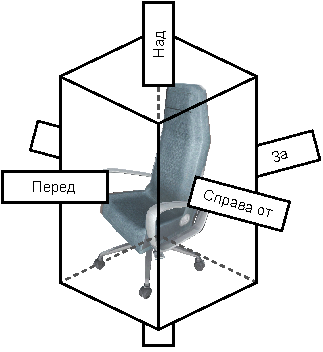
\includegraphics[width=0.8\textwidth]{matmex-diploma-template-master/figures/collider.pdf}
    \caption{Ограничительная рамка вокруг стула разделяет пространство вокруг на шесть зон}
    \label{fig:collider}
  \end{minipage}
  \hfill
  \begin{minipage}{0.45\textwidth}
    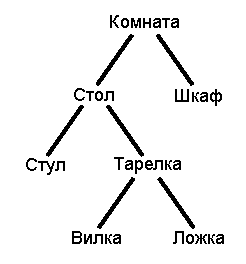
\includegraphics[width=0.8\textwidth]{matmex-diploma-template-master/figures/child_parent_relationship.pdf}
    \caption{Иерархическое представление комнаты}
    \label{fig:room_relationship}
  \end{minipage}
\end{figure}

Также в работе уделяется внимание представлению генерируемых объектов в виде упрощенных фигур. Исследователи пришли к выводу, что прямоугольный параллелепипед является хорошим приближением для многих объектов мебели. В таком представлении каждый предмет имеет ровно шесть граней, что сводит всевозможные случаи расстановки объектов к простым \enquote{перед}, \enquote{за}, \enquote{справа от} и т.~д (рис. \ref{fig:collider}). Наряду с этим авторы рассматривают концепцию детско-родительских отношений между предметами мебели, на вершине которой располагается вся декорируемая комната (рис. \ref{fig:room_relationship}).

\subsubsection{Основанный на правилах подход}

Идеи представления объектов, упомянутые выше, прослеживаются в работе \cite{lidberg2020hierarchical}. Условно их систему можно разделить на две составляющее: входные данные для генерации и сам алгоритм расстановки.

Входные данные определяются таблицей, содержащей сведения о всевозможных предметах мебели и их характеристиках.
Каждой строке соответствуют правила размещения объекта, вероятность его появления в различных пространствах, список предметов, которые он способен породить, и информация о том, является ли объект листовым, т.~e существующем исключительно по запросу родительского объекта. В свою очередь, алгоритм выражается в последовательности из шести шагов: инициализация генератора, выбор объекта, размещение и поиск свободного пространства, размещение листовых предметов и рекурсивный переход к заполнению дочерних пространств. В случае неудачи на некоторых шагах алгоритм способен вернуться на несколько итераций назад и повторить действия, пока положительный ответ не будет получен. Такое поведение может привести к неразрешимым сценариям, при которых время работы алгоритма окажется существенным, но в конечном итоге результат обещает быть более предсказуемым. 

После проведения независимого оценивания стало понятно --- система более чем способна генерировать реалистичные интерьеры. Участникам опроса до конца не сообщалось о целях его проведения, и многие из были уверены, что помогают человеку-дизайнеру подобрать лучшее интерьерное решение.

\subsection{Особенности Unity проекта}

Как было упомянуто раннее, Time Reactor --- это игра, созданная с использованием игрового движка Unity. До этого времени этажи заполнялись уже готовыми экземплярами комнат --- по одному на каждый тип помещения. Задача процедурной генерации интерьера, в свою очередь, заключалась именно в заполнении пустых версий этих комнат без изменения их размера и пропорций. В ином случае следует говорить о \textit{процедурно генерируемом экстерьере}.

Специфика Unity Engine позволяет использовать в игровых скриптах язык семейства .NET --- C\#. Это делает возможным интеграцию в проект библиотек на другом функциональном языке .NET --- F\#. Такой подход позволил отделить генератор от игры и открыл новые перспективы для использования алгоритма в других проектах.  

\subsection{Генератор псевдослучайных чисел}

Генератор псевдослучайных чисел решает проблему сохранения интерьера комнаты при ее повторном посещении. При инициализации на вход генератору поступает число, называемое \textit{random seed} или просто \textit{seed}. Одинаковые входные значения seed гарантируют одну и ту же последовательность чисел, выдаваемых генератором, при каждом запуске программы. 

В качестве псевдослучайного генератора в проекте используется экземпляр класса \texttt{Random} из пространства имен \texttt{System}. Входными данными для него служит номер этажа --- уникальное число, характеризующее каждую из комнат.

Вышесказанное совсем не означает, что помещения обязаны оставаться неизменными и после смерти игрока. Предположим, на третьем этаже в двух различных играх расположилось складское помещение. Интерьер в них будет идентичным --- генератор в обоих случаях задавался цифрой \enquote{3}. Для добавления большей вариативности в интерьерах перед процессом генерации данные для размещения перемешиваются. Схожая система уже используется в Time Reactor при расстановке врагов.
 
% !TeX spellcheck = ru_RU
% !TEX root = vkr.tex

\section{Архитектура решения}

\subsection{Детали реализации SpMSpV}

На платформе .NET существует поддержка параллельных вычислений с использованием асинхронных (т.~e не блокирующих выполнение других процессов) выражений \texttt{tasks}. Они позволяют разбить работу программы на небольшие подзадачи и запустить их параллельно на доступных вычислительных ядрах.

Так как эффективность параллельной версии алгоритма, главным образом, зависит от количества используемых потоков, для векторно-матричных операций были добавлены параметры \texttt{level} --- для сложения и \texttt{multiLevel}, \texttt{addLevel} --- для умножения. Эти аргументы представляют собой \textit{уровни распараллеливания}; к примеру, для ненулевого \texttt{level} функции \texttt{vectorAddition} (листинг. \ref{lst:add}) формируются две задачи, исполняемые параллельно,  для ненулевого \texttt{level -- 1} формируются ещё две подзадачи и т.~д.

\begin{lstlisting}[style=fsharp, caption={Часть функции сложения векторов, отвечающая за параллельную составляющую векторной операции.}, label={lst:add},  frame=single, firstnumber=33]
| BinTree.Node (x, y), BinTree.Node (z, w) ->
    if parallelLevel = 0u then
        let left = treesAddition 0u x z
        let right = treesAddition 0u y w

        if left = BinTree.None && right = BinTree.None then
            BinTree.None
        else
            BinTree.Node(left, right)
    else
        let tasks =
            [| async { return treesAddition (parallelLevel - 1u) x z }; 
            async { return treesAddition (parallelLevel - 1u) y w } |]

        let results = tasks |> Async.Parallel |> Async.RunSynchronously
\end{lstlisting}

\newpage

Аналогично сложению используются \texttt{multiLevel}, \texttt{addLevel} в функции \texttt{multi\-plication}, однако в процессе формируются четыре подзадачи вместо двух (листинг. \ref{lst:multi}). Это различие обусловлено строением вектора и матрицы: узлы дерева, представляющего вектор, имеют ровно два потомка, а узлы дерева, представляющие матрицу --- четыре. Примерная визуализация распределения задач между узлами вектора при сложении представлена на рис. \ref{fig:tree}, а последовательность выполнения операции --- на рис. \ref{fig:uml}.

\begin{lstlisting}[style=fsharp, caption={Часть функции умножения вектора и матрицы, отвечающая за параллельную составляющую векторно-матричной операции.}, label={lst:multi},  frame=single, firstnumber=93]
else
    let multiTasks =
       [| async { return Vector(multiTrees (parallelLevel - 1u) left first,
                  vector.Length) }
          async { return Vector(multiTrees (parallelLevel - 1u) right third,
                  vector.Length) }
          async { return Vector(multiTrees (parallelLevel - 1u) left second,
                  vector.Length) }
          async { return Vector(multiTrees (parallelLevel - 1u) right fourth,
                  vector.Length) } |]

    let multiResults = multiTasks |> Async.Parallel |> Async.RunSynchronously

    let leftTree1 = multiResults[0]
    let leftTree2 = multiResults[1]
    let rightTree1 = multiResults[2]
    let rightTree2 = multiResults[3]

    let addTasks =
       [| async { return (vectorAddition addLevel plusOperation
                  leftTree1 leftTree2).Storage }
          async { return (vectorAddition addLevel plusOperation
                  rightTree1 rightTree2).Storage } |]

    let addResults = addTasks |> Async.Parallel |> Async.RunSynchronously

\end{lstlisting}

\begin{figure}
    \centering
    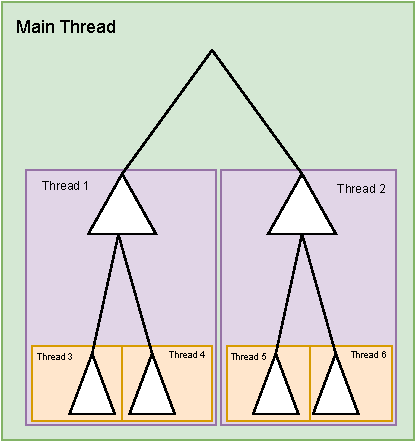
\includegraphics[width=0.6\textwidth]{QuadTree.pdf}
    \caption{Распределение потоков между узлами дерева, представляющего разреженный вектор, при сложении\\}
    \label{fig:tree}
    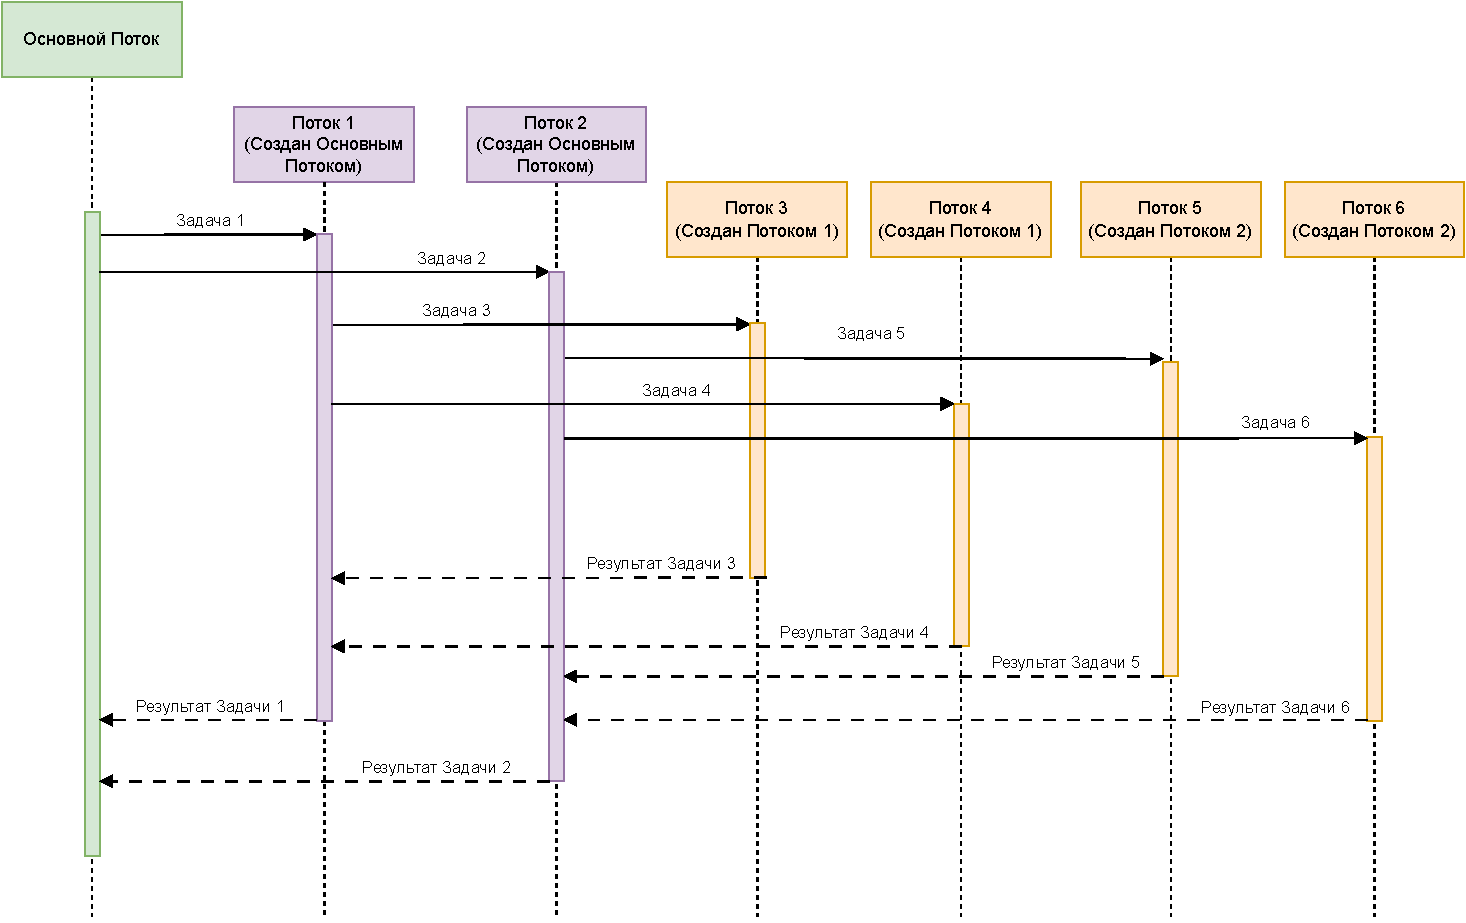
\includegraphics[width=0.9\textwidth]{SequentialUML.pdf}
    \caption{Последовательность выполнения операции сложения векторов с использованием многопоточности}
    \label{fig:uml}
\end{figure}

\subsection{Реализация BFS}

\begin{lstlisting}[style=fsharp, caption={Функция, реализующая обход в ширину с применением матрично-векторных операций.}, label={lst:bfs},  frame=single, firstnumber=32]
let BFS startVertexList (graph: Graph<'Value>) =

   let rec inner (front: Vector<unit>) visited iterationNumber =
      if front.IsEmpty then
          visited
      else
          let newFront = multiplication 0u 0u fPlus fMulti front graph.AdjacencyMatrix

          let front = vectorAddition 0u fPlusMask newFront visited

          let visited = vectorAddition 0u (fPlusVisited iterationNumber) visited front

          inner front visited (iterationNumber + 1u)

   let front = Vector(startVertexList, graph.VerticesCount, ())
   let visited = Vector(startVertexList, graph.VerticesCount, 0u)

   inner front visited 1u
\end{lstlisting}

Алгоритм BFS на листинге. \ref{lst:bfs} в точности реализует шаги 1--4, упомянутые в обзоре. Неочевидным остаётся шаг получения маски; в действительности необходимые действия выполняются в строке 40 без инициализации самой \texttt{mask}.

Функция \texttt{fPlusMask} на листинге. \ref{lst:mask} используется при сложении нового фронта и вектора посещённых вершин --- на месте \texttt{front} получается ненулевое значение, только когда вершину предстоит посетить впервые. 

\newpage

\begin{lstlisting}[style=fsharp, caption={Функция, имитирующая поведение маски для обновления вектора-фронта.}, label={lst:mask},  frame=single, firstnumber=18]
let fPlusMask a b =
    match a, b with
    | Some _, Option.None -> Some()
    | _ -> Option.None
\end{lstlisting}


% !TeX spellcheck = ru_RU
% !TEX root = vkr.tex

\section{Апробация}

Вопросы для апробационного исследования были отобраны согласно критериям методики оценки качества продукта System Usability Scale (SUS). В опросе приняли участие 13 человек. Предлагаемые формулировки и результаты исследования представлены в табл. \ref{tbl:results}.

Средний балл среди участников опроса по системе SUS составляет 68,1 при среднем показателе в 68 для систем, использующих данную систему оценивания. Все участники тестирования отметили: генератор быстро справляется с расстановкой и не создает больших задержек во времени. Полученные данные показывают, что система хорошо справляется с поставленной задачей на устройствах различных конфигураций. Более половины опрошенных не смогли с уверенностью ответить о наличии или отсутствии комнат, заполненных вручную. Такой результат может свидетельствовать о высоком уровне реалистичности игровых интерьеров.

\begin{landscape}
\begin{table}
\begin{center}
\caption{Апробационные вопросы и процент участников, выбравших предложенные варианты}
\label{tbl:results}
\rowcolors{2}{black!2}{black!10}
\scalebox{0.5}{
\begin{tabular}{|l|с|с|с|с|с|}
\hline
Вопрос &  Полностью не согласен & Скорее не согласен & Затрудняюсь ответить & Скорее согласен & Полностью согласен\\
\hline
\hline
Интерьеры комнат разнообразны.  & 0,0  & 0,0 & 0,0 & 53,9 & 46,1 \\
Комнаты выглядят пустоватыми.   & 61,5 & 15,4 & 23,1 & 0,0  & 0,0 \\
Я могу свободно перемещаться по комнатам.& 0,0 & 0,0 & 0,0 & 61,54  & 38,46 \\
Мне не нравится общее визуальное оформление комнат. & 61,5 & 30,8 & 7,7 & 0,0 & 0,0 \\
Количество реалистичных комнат превышает количество нереалистичных. & 0,0 & 0,0 & 8,3 & 25,0 & 66,7 \\
Время генерации интерьера не приемлемо. & 92,3 & 7,7 & 0,0 & 0,0 & 0,0 \\
Иерархические паттерны выдержаны хорошо. & 0,0 & 0,0 & 0,0 & 15,4 & 84,6 \\
Генератор не справляется с заполнением больших пространств. & 84,6 & 15,4 & 0,0 & 0,0 & 0,0 \\
Мебель расставлена реалистично. & 0,0 & 0,0 & 0,0 & 69,2 & 30,8 \\
Я уверен, что в игре не было заполненных вручную комнат. & 38,5 & 23,1 & 23,1 & 0,0 & 15,4 \\
\hline
\end{tabular}
}
\end{center}
\end{table}
\end{landscape}
% !TeX spellcheck = ru_RU
% !TEX root = vkr.tex

\section*{Заключение}

В рамках выполнения данной работы были получены следующие результаты.

\begin{itemize}
\item Реализованы тип-матрица и тип-вектор с использованием деревьев квадрантов в качестве метода хранения разреженных структур, а также векторно-матричные операции над ними.
\item Реализован алгоритм обхода графа в ширину с использованием линейной алгебры.
\item Реализованы параллельные версии векторно-матричных операций с помощью выражений \texttt{async} --- специальной конструкции языка F\#.
\item Выполнено экспериментальное исследование реализованного алгоритма. Обход в ширину с использованием параллельной версии матрично-векторных операций показал ускорение до 3.45 раз на матрицах среднего размера в сравнении с однопоточной версией и не показал себя эффективно на матрицах малого и большого размеров.
\end{itemize}

Результаты исследования могут иметь практическое применение в областях, где требуется анализ разреженных графовых данных. 

\setmonofont{CMU Typewriter Text}
\bibliographystyle{ugost2008ls}
\bibliography{BFS_report_Savelyeva_Polina}
\end{document}
